
\chapter{Introduction}
\label{chap:intro}
%%%%%%%%%%%%%%%%%%%%%%%%%%%%%%%%%%%%%%%%%%%%%%%%%%%%%%%%%%%%%%%%%%%%%%%
%%%%%%%%%%%%%%%%%%%%%%%%%%%%%%%%%%%%%%%%%%%%%%%%%%%%%%%%%%%%%%%%%%%%%%%
%%%%%Overview%%%%%%%%%%%%%%
%%%%%%%%%%%%%%%%%%%%%%%%%%%%%%%%%%%%%%%%%%%%%%%%%%%%%%%%%%%%%%%%%%%%%%%
%%%%%%%%%%%%%%%%%%%%%%%%%%%%%%%%%%%%%%%%%%%%%%%%%%%%%%%%%%%%%%%%%%%%%%%

\section{Prelude}
\label{sec: overview}
%what do we have inside galaxies:
% stuff we don't care about because they don't have a big contribution on the SED 1) planets; 2) black holes 3) dark matter
Inside every galaxy, there are millions of stars, planets, and black holes, as well as dust and gas.
They all affect each others' formation, evolution, and extinction.
There is also dark matter inside every galaxy, which, to the best of our knowledge, only has gravitational effects on the other components.
Nearly all the information we can obtain from galaxies other than our own comes from their light.
Since each observable phenomenon inside galaxies emits most of its energy in specific wavelengths, 
a plot of brightness/flux density of galaxies as a function of wavelengths, which is called spectral energy distribution (SED), is a useful tool to gain a information about galaxies. 
Young and evolved stars, dust, and gas in the space between the stars are the most important contributors to the SEDs of galaxies.
Planets and black holes without an accretion disc, on the other hand, have a much lower intensity compared to the other aforementioned components, and therefore contribute less to the SED.
Therefore, with properly modeling observed features in SEDs we can extract information about the evolution of stars, dust, and gas inside galaxies.

%stars
Arguably, stars are the main component of normal galaxies.
They control the chemical composition and structure of galaxies by transforming gas into new stars and by transforming dead stars back into gas.
They are also central to the formation and evolution of planetary systems.
The energy provided by stars is necessary to create and maintain the life on planets. 
The study of the formation and evolution of the Sun, and more generally that of stars, helps us understand more about our origin and the future of our Solar System.
Furthermore, in order to completely understand the formation and evolution of galaxies from early universe to the current epoch, the knowledge of the formation and evolution of stars is necessary. 
As a result, the study of stellar formation and evolution has been a central topic in astronomy and astrophysics for decades.

%ISM 1)Gas 2)dust
%There could be a galaxy without stars (i.e. dark galaxies~\citep[][and references therein]{Cantalupo12}), but there will never be a galaxy without gas. %: this is a very strong statement. Some galaxies, like dwarf ellipticals, are pretty gas-free (at least now). So qualify this a bit. done
Among observable objects in galaxies, gas has a crucial role in formation and evolution of galaxies.
Gas and dust in galaxies can be found in the space between stars.
This space is called the interstellar medium (ISM), and is full of low density gaseous clouds with neutral or ionized atoms and/or molecules, and microscopic dust grains.
The gas and dust in the ISM are heated by interstellar radiation field and cool through a variety of line and continuum processes which usually depend on the local physical conditions. 
The effect of the ISM on stellar formation is undeniable; it provides the raw material for the formation of stars~\citep[e.g.][]{Kennicutt08,Bigiel08}.
Studying the interstellar medium is not only essential to understanding the formation of stars, but also it is necessary for interpretation of stellar evolution due to fact that stars release their material into ISM when they reach the end of their evolutionary track.

In a galaxy, like our own, star formation begins with the condensation of giant molecular clouds (GMCs, $\sim 10^7$ M$_{\odot}$) in the ISM due to gravitational instabilities. 
The denser regions within GMCs collapse under their own gravity, self-gravity, and creates clumps.
Some of these clumps, which have a similar distribution to stellar initial mass function (IMF), develop into self-gravitating cores.
Then these clumps continue to become denser and transfer to protostars. 
Since the protostars have a higher mass than their surroundings, more gas from GMCs add to protostars.
This procedure continues until hydrogen burning in centre of protostars starts (see~\cite{McKee07} for more detail). 

Metallicity, which is defined as the ratio of abundance of metals (any element heavier than hydrogen and helium) to the abundance of hydrogen, affects formation and evolution of stars indisputably.
\cite{Walch11} showed that in the case of large scale turbulence, the effect of metallicity on star formation is negligible, but if turbulence is decaying,  metallicity has a strong impact on stabilizing self-gravitating cores.
Metals also play an important role in heating, cooling, and ionizing processes in the ISM.
Since cooling is one of the main reasons for condensation of GMCs~\citep[e.g.][]{Maio07}, in low metallicity regions star formation may be suppressed. 
The amount of metals in stars also affect their evolutionary tracks~\citep[e.g.][and references therein]{Maeder02}.
For instance, low metallicity stars tend to be have lower mass loss by stellar wind than that with higher metallicity.
Observation shows that massive low metallicity stars rotate faster.
Being more massive at the end of evolutionary track makes massive low metallicity stars have a lower chance to explode and become a supernova.


%what does SED look like?
Our primary source of information about galaxies, specifically unresolved ones, is their spectral energy distributions. 
Broadly speaking, young and hot stars emit most of their light in ultraviolet (UV) wavelengths, evolved stellar populations show themselves in optical and near-infrared (NIR) emission, and gas and dust heated by stellar emission are bright in mid-infrared (MIR) or far-infrared (FIR) wavelengths.
Therefore, UV-to-IR SEDs contain valuable information about galaxies' stellar evolution and their ISM. 
Other wavelengths regimes in galaxy SEDs (e.g. X--ray, radio), that are dominated by processes such as active galactic nuclei, quasars, and supernovae shocks, are beyond the scope of this thesis.
The general shape of SEDs mirrors the morphological type of galaxies; starburst galaxies, which have high star formation rates (SFRs), emit the bulk of their energy in the UV, while the light of quiescent galaxies is dominated by optical and IR emission. 
Detailed information about the age of stellar populations and other properties of galaxies can be determined by modelling their SEDs.

 %how do you model it? %SED model CIGALE %Population synthesis ----> SFR, stellar mass 
The stellar population synthesis method, which sums stellar spectra of a galaxy to produce its spectrum, has been widely utilized since the 1970s~\citep[e.g.][]{Tinsley72,Searle73} to model SEDs of galaxies.
A thorough SED model must include stellar population models~\citep[e.g.][]{Bruzual93,Bruzual03,Maraston05}, stellar emission and dust attenuation~\citep[e.g.][]{Calzetti00,Dopita05}, dust grain emission such as from polycyclic aromatic hydrocarbons~\citep[PAHs; e.g.][and references therein]{Tielens08}, and IR emission from gas and dust~\citep[e.g.][]{Chary01,Dale02,Lagache03,Lagache04,Smith07a,Draine07}.
Many groups have modelled SEDs for different types of galaxies and created SED templates (for more information see the review of \cite{Walcher11} on fitting of SEDs and references therein).
Since the physical parameters of templates generated by the SED models are known, we can find properties of observed galaxies by fitting their SEDs, (either by minizing $\chi^2$ or by Bayesian analysis)  using the templates.
One example of an SED-fitting code is {\em CIGALE}: Code Investigating GALaxy Emission~\citep{Noll09}.
It combines SED models and uses Bayesian analysis to find the best-fit SED for observed data in the rest-frame UV-to-IR.
Some of the physical properties of gaalxies should be assumed as an input data to find the best SED, and others will be derived from SED results~\citep[See][for more detail]{Walch08}.
For example, the Best fitted SED has information regarding star formation history and stellar mass to light ratio.
By integrating star formation history over a specific time scale, SFR can be derived. 
knowing the stellar mass to light ratio, one can use the observed luminosity to calculate stellar mass in galaxies.

Formation of stars in galaxies depends on many parameters such as gas, stellar mass, metallicity, dust, galaxy's morphology, and location of the star forming region inside the galaxy.
In extragalactic astronomy, measuring the rate that stars form is uncertain and relies upon theoretical models and observational data.
Studying star formation and its relation to other quantities in galaxies in an ongoing research.
In this chapter, we present a review of observational methods of measuring the star formation rate and the main properties that affect measuring and scaling the SFR. A discussion of the ISM and its role in star formation is presented in $\S$~\ref{sec: ism_intro}. In $\S$~\ref{sec: sfr_intro} we discuss measuring the star formation rate, followed by a discussion of the measurement of the stellar mass in $\S$~\ref{sec: starmass_intro}. Current issues about star formation and its relation to other properties of a galaxy are discussed in $\S$~\ref{sec: pre_intro}. 
%% We or I?!


%%%%%%%%%%%%%%%%%%%%%%%%%%%%%%%%%%%%%%%%%%%%%%%%%%%%%%%%%%%%%%%%%%%%%%%
%%%%%%%%%%%%%%%%%%%%%%%%%%%%%%%%%%%%%%%%%%%%%%%%%%%%%%%%%%%%%%%%%%%%%%%
%%%%%ISM%%%%%%%%%%%%%%
%%%%%%%%%%%%%%%%%%%%%%%%%%%%%%%%%%%%%%%%%%%%%%%%%%%%%%%%%%%%%%%%%%%%%%%
%%%%%%%%%%%%%%%%%%%%%%%%%%%%%%%%%%%%%%%%%%%%%%%%%%%%%%%%%%%%%%%%%%%%%%%


\section{Components of the Interstellar Medium} 
\label{sec: ism_intro}
%how do we observe it
%what the observation tell us
% how do we measure the dust and gas
The interstellar medium in galaxies is a complex system with a wide range of structures, but these structures can be divided into two main components: gas and dust.
The gas in the ISM of galaxies is mostly made of hydrogen and helium, with 1 per cent heavier elements (metals), and can be in the form of clouds or diffuse (diffused?) regions.
Gas clouds include molecular clouds, cold neutral atomic hydrogen (\hi) or hot \hi~clouds, and diffuse gas can be either \hii~(ionized hydrogen) regions or hot intercloud medium.
Dust mostly contains silicate, and graphite grains can be seen in dark clouds or galactic cirrus.
Emission lines from atoms or ions (i.e \hii~regions) in a hot gas, lines from molecules in cold clouds, and 21~cm emission of \hi~are the main observable signatures of gas in the ISM of galaxies.
Dust can be observed directly through far-infrared and sub-millimeter wavelength emission or indirectly through its extinction and attenuation effects (see Sec.~\ref{sec: extinction}).

Molecular clouds in the ISM are cold ($\sim10$ K) and dense ($ 50<n<500$ cm$^{-3}$); masses of molecular clouds range from a few to millions of solar masses~\citep{Bolato08}.
Density in the molecular clouds is not uniform. There are dense and colds clumps inside these clouds.
Since these clumps are ideal places to form stars, studying molecular clouds has an important role in understanding formation of stars
However, H$_2$ molecules, the main component of molecular clouds, have no permanent electric dipole moment which makes them difficult to detect.
The second dominant component, helium, is a mono-atomic gas and has the same problem as hydrogen, but these clouds also contain heavier elements such as carbon monoxide, hydrogen cyanide, water, ammonia and more than tens of others.
Carbon monoxide (CO) molecules are the third-most abundant constituent of molecular clouds.
In fact, most of our knowledge from molecular clouds comes from observing line emission of CO molecules, which {\bf due to their heavy weight, they have very low energy rotational state} and can be excited in the temperature of molecular clouds.%%Sr: I'll add more detail here
Other heavier molecules have emission lines which are also detectable in the spectrum of clouds (specially galactic ones), but observing CO emission is the most common way to study the properties of molecular clouds i.e. their mass (see Sec.~\ref{sec: ismmap} for more details).

The molecular clouds are surrounded by clouds of atomic gas~\citep{Kennicutt12}, which are easily traceable by 21-cm emission.
Hydrogen atoms in the ISM (excluding the regions close to hot stars, see below) are in their ground state. 
The electron and proton spins in the ground state can be parallel (i.e. both spin up) or anti-parallel (i.e. the proton's spin is up and the electron's spin is down or vice versa). 
The energy of the anti-parallel mode is slightly less than the parallel mode.
Since atoms always want to be in the state with lowest energy possible, electrons in the parallel mode have a tendency to flip to the anti-parallel mode. 
However, the difference between these two states is very small and it takes millions of years before the transition happens.
The large amount of hydrogen atoms compensates for the rareness of the transition and at any given time, there are enough hydrogen atoms to emit the 21-cm radiation. 
Observation of the \hi atoms is specifically necessary for understanding physical properties and dynamics of the ISM, which leads to understanding the star formation process~\citep{Walter08}.

\hii~regions are hot and low density regions that are mostly located in the disks of spiral galaxies.
High energy UV photons emitted by massive new born stars have sufficient energy to ionize their surrounding gas, and
~\halpha emission is the main observable feature of \hii~regions.
The temperature and density of these regions can be estimated by observing other recombination lines such as H$\beta$, and forbidden lines such as \sii, \oii, \oiii, and \nii. 
Forbidden lines are not called so because there is no chance of them occurring, but merely because their probability is much lower than the normal ``allowed'' transitions.
Optically bright \halpha emission from \hii~regions is correlated with number of new massive stars in regions, and can be used as a star formation tracer~\citep[e.g.][]{Kennicutt98b,Calzetti13}.
Studying \hii~regions provides valuable insight into star forming regions by providing information such as star formation rate, initial mass function (IMF), and distribution of ionizing stellar masses~\citep[][and references therein]{Azimlu11}.


Dust has an insignificant effect on the mass of the ISM, but it plays crucial roles in the ISM's evolution.
%The total gas mass of galaxies can be determined using optical depth in sub-mm waveband of dust emission. 
In spiral galaxies, dust grains are located in cold regions ($\sim$30~K) and have a power-law size distribution.
The source of thermal emission of dust is from stars, and shape of the continuum depends on size of the grain.
Mid-infrared emission from dust grains is mainly dominated by PAHs heated by evolved stellar population~\cite{Smith07a} or recently formed intermediate-mass young stars~\cite{Peeters04}. 
Large grains that are either heated by light from star-forming regions or by the interstellar radiation field from total stellar population emit most of their light in far-infrared~\citep[e.g.][]{Calapa14, lu14}
Dust is the main source of extinction and reddening of starlight (See Sec.\ref{sec: extinction} for more information).

\subsection{Mapping the Interstellar Medium} 
\label{sec: ismmap}
Measuring the mass of gas in galaxies is a necessary step to knowing how much raw material is available for forming stars.
A map of the total gas mass in the ISM can be produced by direct observations of gas or using interstellar dust as a tracer. 
Neutral atomic and molecular hydrogen are the most common components of the ISM. 
Therefore, to produce a total gas mass map in galaxies, maps of these two components can be added together and multiplied by a constant factor to account for heavier elements, which are mostly helium and cannot be observed directly. 
Another way to do the mapping is to assume that the ratio of total gas to dust is constant across the galaxy, and convert dust observations to a map of total gas mass.

\subsubsection{Direct Measurement of the Gas}

The surface density of gas in the ISM of galaxies can be measured by direct observation of the neutral and molecular hydrogen.
This method can be promising if observational data with resolved molecular and atomic clouds are available.
However, given the state of the current technology, having high resolution images of clouds for most galaxies is not possible. 
This problem shows itself for distant galaxies more than nearby galaxies. 
As a result, using images of molecular and atomic cloud to measure surface density of gas in ISM is limited to the telescopes resolution. 
 
%\subsubsection{Molecular Clouds}
%PB: some repetition from earlier subsection here. 
The carbon monoxide molecule has a weak permanent electric dipole moment and a ground rotational transition with low excitation energy. 
Given its low energy and critical density, CO can easily be excited even in cold molecular clouds.
Therefore, CO (usually the $J(1\rightarrow 0)$ rotational transition, observed at 2.6 mm) is used as a tracer of the mass of molecular clouds dominated by molecular hydrogen~\citep[e.g.][] {Sanders84}.
Higher rotational transitions of CO can be used as a tracer as well, but they are not as common as $J(1\rightarrow 0)$.

\cite{Young91} described the relationship between the CO luminosity of a cloud and its mass. The CO luminosity of a cloud is:
\begin{equation}
L_{CO} = D^2 \int I_{\rm CO} d\Omega, 
\end{equation}
%NOTE: Equations must be punctuated.%
where $D$ is the distance to the cloud and $I_{\mathrm CO}$ is the CO brightness temperature integrated over the line profile in KKms$^{-1}$.
It can be written as ${\int T_{\mathrm CO} dV}$ where $T_{\mathrm CO}$(k) is the peak brightness temperature in the CO line and $V$ is the line-width in Kms$^{-1}$.
For a uniform cloud with a radius $R$, the CO luminosity is given by:
 \begin{equation}
L_{\rm CO} = \pi R^2 T_{\rm CO} \Delta V.
\end{equation}

Giant molecular clouds are self-gravitating systems~\citep[e.g.][]{Efstathiou83,Blitz99}.
Thus, using the virial theorem leads to calculating the mass of the cloud: 
\begin{equation}
 \label{equ: vir}
 M_{cloud} = L_{\rm CO} \sqrt{\frac{4\rho}{3\pi G T_{\rm CO}}},
\end{equation}
where $\rho$ is the mass density of the cloud and $\sqrt{\frac{4\rho}{3\pi G T_{\rm CO}}}$ is called the conversion factor.
Equ.~\ref{equ: vir} shows that the total mass of molecular clouds and the CO luminosity of the cloud are directly related~\citep{Young91}. 
Since the dependency of $I_{\mathrm CO}$ to optical depth is negligible~\citep{Krumholz09}, total CO luminosity of the galaxies can be used to measure the total H$_2$ mass of galaxies.
The relation between CO emission and H$_2$ cloud mass is shown to be
\begin{equation}
N_{\rm H_2}/\rm cm^{-2} = X_{\rm CO} \times I_{\rm CO}/{\rm K km s}^{-1},
\end{equation}
where X$_{\rm CO}$ is the conversion factor (also known as the X-factor).
The X-factor is different for each galaxy and sometimes is even different in regions within a galaxy due to differences in properties such as metallicity.
Although assuming a constant conversion factor for galaxies like M82 and M31 can lead to accurate estimation of global molecular gas mass, in regions with low metallicity this assumption leads to uncertainties~\citep{Bolato13}. 
Various groups are working on observations of different types of galaxies to measure the X-factor for them~\citep{Wilson95, Bosselli02, Bolato13}.

\begin{figure}
\label{fig: mco}
\centering
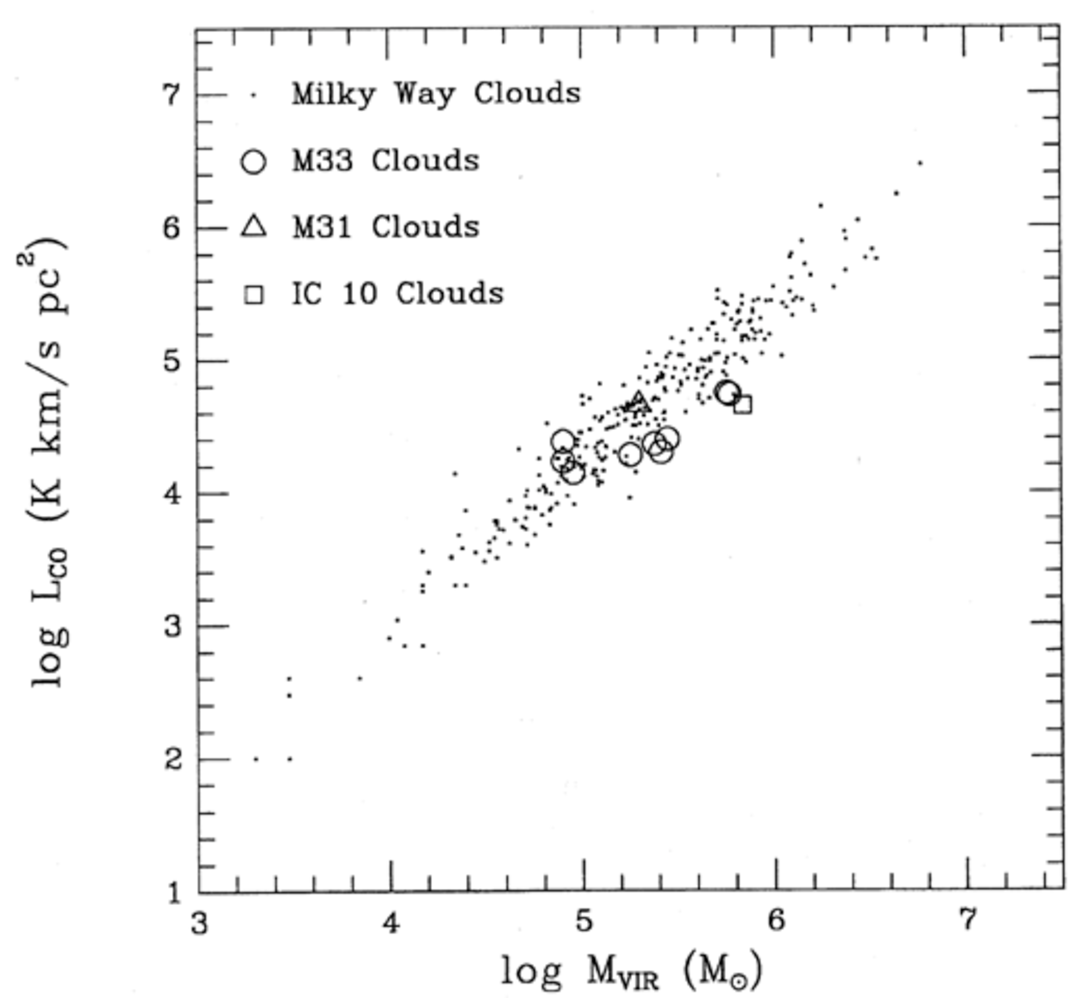
\includegraphics[width=16cm]{../image_intro/mvirial_lco.pdf}
\caption{Relation between the virial mass and CO luminosity for the Milky Way (dots), M33 (open circles), M31 (triangles), and IC~10 (squares) clouds. Virial masses are measured from selected high spatial resolution CO observations. The extragalactic molecular clouds are very similar to those in the Milky Way. Adapted from~\cite{Young91}.}
\end{figure}

In order to empirically determine the relation between H$_2$ masses and CO luminosities, many observational attempts have been made on both Galactic and extragalactic scales. 
One of the most significant studies in this regard was done by~\cite{Solomon87}, who studied this relation over more than 273 clouds inside the Milky Way and found a strong correlation between the virial mass of molecular clouds and CO luminosity. 
In Local Group galaxies, several groups have measured size, line width, and CO luminosity of molecular clouds and investigated the relation between  their virial masses and CO emission in environment other than the Milky Way. 
Pioneering works in measuring the extragalactic conversion factor were done for M31 and M32~\citep[e.g.,][]{Wilson89, Wilson90}. 
Fig.~\ref{fig: mco} shows the CO luminosity verses virial masses of molecular clouds in the Milky Way, M31, M33, and IC~10. 
The extragalactic molecular clouds are similar to those in the Milky Way. 
The conversion between the CO luminosity and H$_2$ masses is still a controversial topic~\citep[e.g.][]{Narayanan11, Bolato13, Sandstrom13}.
Problems regarding metallicity are not yet resolved and it is still not clear whether the conversion factor is global or local. 
Extragalactic investigations were limited to nearby galaxies due to technical problems regarding resolution and sensitivity of the telescopes. 
To measure the clouds in distant galaxies, spatial resolution of maps must be better than 40 pc which is the typical size of a giant molecular cloud~\citep[e.g.][and refrences therein]{Young91,Bolato13}. 


%%%to be conticued